\documentclass[../dissertation.tex]{subfiles}
\begin{document}

\chapter{Testing and Evaluation}
\label{chap:testing-eval}

\section{Testing}

\subsection{Unit Testing}

Unit tests have the purpose of testing each individual component of the application for expected behaviour \cite{runeson2006survey}. Unit testing was conducted on the two main components of the Tulip Web Wrapper, along with on the Django \texttt{views} responsible for returning the HTML to the client. 

\subsubsection{Conversion from \texttt{.tlp} to \texttt{.json}}

To confirm that the conversion from a Tulip network to a JSON object was successful, tests were created for several different networks. The test set up included loading three network from a file into memory using Tulip's \texttt{tlp.loadGraph()}. Then, on each of the networks, the conversion code was run and it was confirmed that the number of nodes and edges was correct, with the function \texttt{TlpJsonConverter.tlp\_to\_json()}.

\subsubsection{Confirming that each bundling algorithms work}

To test each algorithm initially three different networks were loaded into the system using the Tulip function \texttt{tlp.loadGraph()}. One of these networks would be used to test node bundling based on cliques, since it was a very interconnected network. The other two networks would be used to test node pruning and node bundling based on number of edges, being far more sparsely connected networks. Each test consisted of checking the number of nodes upon loading in the network, applying the appropriate operation that was being tested for, and then confirming that the number of nodes and edges returned from the function was as expected.

\subsubsection{Successful page responses}

The unit tests, which confirmed that both the part of the back-end that returned data to the front-end, worked by creating a fake call to the server using a GET or POST request as expected and that the Tulip Web Wrapper worked as appropriate. This was done by checking that the calls were successful and either returned a status code of 200 if a \texttt{HttpResponse} was returned, or included success = True if a \texttt{JsonResponse} was returned.

\subsection{Integration Testing}

Integration tests serve the purpose of testing that each component works predictably when combined with all other components it should work with \cite{basanieri2000practical}. For this project, they serve the purpose of confirming that the Tulip Web Wrapper worked as expected, and that it interacted with the rest of the back-end correctly.

The integration tests for the Tulip Web Wrapper involved creating a network in the database during the set up phase of the test, and then loading in that network using different algorithms and ensuring the output at the end was correct. This entailed calling the \texttt{loadGraph} API endpoint using JavaScript AJAX \cite{jquery-ajax} and passing in appropriate parameters such as the network name, and whether node pruning or node bundling using number of edges was enabled. The response of that call (a JSON object) was then decoded and it was checked if the call had been successful, and if it had contained the correct number of nodes and edges, along with the expected number of nodes that had been pruned of bundled. This ensured that the logic within the view was correct, that the bundling code worked as anticipated, and that the conversion worked correctly.

\section{User Evaluation}

As stated in Chapter \ref{chap:motiv}, during background research for the project, it was found that the majority of what little there was on massive network visualisation focused on the interface design and quality of interaction between a user and the system. It was hence decided that the aim of this project would be to create a system that enabled users to visualise massive networks within a browser whilst specifically focusing on the performance of the system. This was completed by applying one (or several) algorithm to the network in order to: reduce its size, speed up render times and improve network transfer rates. An additional goal was to ensure that the Tulip Python API Web Endpoint and the JavaScript library were as flexible as possible, to ensure the easy development of future interfaces.

The interface made for this project was kept simple to allow for maximal development time to be spent optimising and testing the web wrapper (it can be seen in Figure \ref{fig:topbar}). Additionally, the JavaScript network visualisation framework used (Vis.js) was chosen due to it's simplicity, and it is known to be less flexible than other choices, such as D3.js - and hence if interface design had been a priority then another framework would have been chosen. 

Given all of the above facts, it was decided that a user evaluation was not appropriate for the project, as significant development time was not spent on the interface. The focus of the project was to make the server and client as high performing as possible. The performance is evaluated in Section \ref{sec:perf-eval}.

\section{Performance Evaluation}
\label{sec:perf-eval}

\subsection{Aim}

The goal of the performance evaluation was to thoroughly test the system that had been created. This would involve loading several different networks into the system, and then recording the performance of the system when different algorithms are used and comparing the results, providing a quantitative evaluation.

\subsection{Methodology}

As SAS had provided four different networks of varying sizes, these would be used evaluate the system. The networks had approximately thirty, two hundred, one thousand and three thousand nodes respectively, and each had approximately the same number of edges as nodes. Each of these networks would first be uploaded into the system and then rendered with the following parameters: no algorithm set, node pruning, node bundling based on number of edges and both node pruning then node bundling based on number of edges. 

It is worth noting that node bundling based on cliques was not tested as it had no effect on the data provided by SAS due to the tree-like structure of the data.

The runs were conducted on the same machine, one by one, while no other application was running apart from the Django development server which hosted the site. Each run of the evaluation was done five times so a reliable average could be taken. For each run, the following information was collected:

\begin{itemize}
    \item Client-Side:
    \begin{itemize}
        \item \textbf{The time taken between the user clicking `Load' and the client getting an AJAX response back.} This was recorded to discover how long the JavaScript took to respond, call the server using AJAX, and get a response - essentially recording the time spend processing the network and sending it across the network.
        \item \textbf{The time spent processing the data got from the AJAX call and formatting it for Vis.js.} This was recorded in order to find out how long it took for JavaScript to process the data and format it appropriately for Vis.js, which included adding all of the nodes and edges to a list and then setting properties (such as size, shape and colour) appropriately.
        \item \textbf{The time spent creating the Vis.js network.} How long it took to create the network in memory from the list of nodes and edges, and any \texttt{options} parameters set.
        \item \textbf{The time spent rendering the network.} How long it took for the visualisation to display. This involves Vis.js creating all of the nodes, positioning them in a circle, and then applying the selected physics model and waiting for the network to settle before it is displayed.
    \end{itemize}
    \item Server-Side:
    \begin{itemize}
        \item \textbf{The time taken to load in the requested \texttt{.tlp} file from the database into Tulip.} This represents how long it took for the network to be located in the database, loaded in to memory and then loaded in to Tulip as a network object.
        \item \textbf{How long pruning the network took.} If applicable, the length of time taken to loop over the network and prune it as appropriate, and return both the modified network and a list containing each node that has been pruned as well as noting how many nodes have been removed from it.
        \item \textbf{How long node bundling based on the number of edges took.}  If applicable, the time taken to decide which nodes should be bundled and to then bundle them, whilst tracking how many nodes have been removed from each bundled node.
    \end{itemize}
    \item Network Information:
    \begin{itemize}
        \item \textbf{The number of nodes in the network.}
        \item \textbf{The number of edges in the network.}
        \item \textbf{How many bytes the packet contains that is to be sent across the network.}
    \end{itemize}
    \item Total Time:
    \begin{itemize}
        \item \textbf{The total time taken from the user clicking `Load' to the network rendering.}
        \item \textbf{The standard deviation of the total time.}
    \end{itemize}
\end{itemize}

\subsection{Results and Discussion}

The following four tables show the effect of different algorithms on different networks. Each table shows the total time taken to load, manipulate and render the network, and how much data was sent. Table \ref{table:30-nodes} shows the results for a network with thirty nodes, Table \ref{table:200-nodes} shows the results for two hundred nodes, Table \ref{table:1000-nodes} shows the results for one thousand nodes and Table \ref{table:3000-nodes} shows the results for three thousand nodes. 

Each percentage in the following sections is created by comparing the time or packet size of the stated algorithm(s) - which are either node pruning, node bundling based on number of edges, or both - against not applying any algorithm.

\subsubsection{30 Nodes}

For a network with approximately 30 nodes, node pruning resulted in a 50\% decrease in total time to visualise, and 36\% decrease in packet size. node bundling based on the number of edges resulted in a 24\% decrease in time to generate and render, and 36\% decrease in packet size. Applying both node pruning and node bundling based on number of edges resulted in a 63\% decrease in amount of time to visualise and a 40\% decrease in packet size. Node pruning is clearly more effective than node bundling, providing lower packet sizes and faster network loading times.

\begin{table}[H]
\centering
\begin{tabular}{|l|l|l|l|l|}
\hline
                    & \textbf{None}    & \textbf{Pruning} & \textbf{Edge-based Bundling}    & \textbf{Both}   \\ \hline
Total Time (ms)     & 170.8 $\pm$ 15.3 & 85.8 $\pm$ 20.5  & 129.6 $\pm$ 19.3 & 63.2 $\pm$ 15.2 \\ \hline
Packet Size (bytes) & 1300             & 827              & 1012             & 785             \\ \hline
\end{tabular}
\caption{Total Times to load a network of 31 nodes and 26 edges, and the size of the packet transferred over the network}
\label{table:30-nodes}
\end{table}

\subsubsection{200 Nodes}

For approximately 200 nodes, node pruning provides a 91\% decrease in total load time and a 49\% decrease in packet size. For node bundling based on number of edges, the decrease in load time was 9\% and the packet size decreased by 20\%. Applying node pruning followed by node bundling based on number of nodes resulted in a 98\% decrease in loading times and a 70\% decrease in packet size. node pruning is again more effective at lowering the amount of data that needs to be transferred and lowering the amount of time to manipulate and render the network.

\begin{table}[H]
\centering
\begin{tabular}{|l|l|l|l|l|}
\hline
                    & \textbf{None}       & \textbf{Pruning}  & \textbf{Edge-based Bundling}       & \textbf{Both}    \\ \hline
Total Time (ms)     & 7382.8 $\pm$ 2010.2 & 663.0 $\pm$ 187.0 & 6749.0 $\pm$ 1075.0 & 146.6 $\pm$ 14.5 \\ \hline
Packet Size (bytes) & 7600                & 3900              & 6100                & 2300             \\ \hline
\end{tabular}
\caption{Total Times to load a network of 199 nodes and 199 edges, and the size of the packet transferred over the network}
\label{table:200-nodes}
\end{table}

\subsubsection{1000 Nodes}

When the network with approximately 1000 nodes was used, similar results to above were seen. There was an 84\% decrease in loading times and 51\% decrease in packet size for node pruning, and a 36\% decrease in loading times and a 29\% decrease in packet size. When applying both node pruning and then node bundling based on the number of edges, the decrease in loading times was 99.997\% and the packet size was reduced by 70\%. Again, node pruning was shown to be more effective than node bundling based on number of edges, but additionally there was a massive decrease in loading times when applying both algorithms. It is hypothesised that the reason such an increase in performance was seen was due to the structure of the network lending itself well to being Node Pruned and then Node Bundled based on number of edges, and hence there was a massive reduction in nodes and edges to be rendered.

\begin{table}[H]
\centering
\begin{tabular}{|l|l|l|l|l|}
\hline
                    & \textbf{None}        & \textbf{Pruning}    & \textbf{Edge-based Bundling}        & \textbf{Both}    \\ \hline
Total Time (ms)     & 59924.4 $\pm$ 8343.5 & 9417.8 $\pm$ 2223.1 & 38139.8 $\pm$ 9383.0 & 152.6 $\pm$ 30.5 \\ \hline
Packet Size (bytes) & 41400                & 20300               & 29400                & 12400            \\ \hline
\end{tabular}
\caption{Total Times to load a network of 1089 nodes and 1087 edges, and the size of the packet transferred over the network}
\label{table:1000-nodes}
\end{table}

\subsubsection{3000 Nodes}

For the largest network, with approximately 3000 nodes, the following results were obtained. Loading times decreased by 81\% and packet size decreased by 44\% for node pruning. For node bundling based on number of edges, a decrease of 48\% was seen for loading times and a 27\% decrease was seen for packet size. When applying node pruning followed by node bundling based on number of edges the decrease in total time was 94\%, and the decrease of packet size was 72\%. Similar to above, a performance increase was most notable for node pruning. 

\begin{table}[H]
\centering
\setlength{\tabcolsep}{0.4em}
\begin{tabular}{|l|l|l|l|l|}
\hline
                    & \textbf{None}          & \textbf{Pruning}     & \textbf{Edge-based Bundling}         & \textbf{Both}        \\ \hline
Total Time (ms)     & 252849.2 $\pm$ 32862.0 & 48956.8 $\pm$ 3937.0 & 131606.6 $\pm$ 6031.3 & 14532.8 $\pm$ 3341.0 \\ \hline
Packet Size (bytes) & 114000                 & 63500                & 83500                 & 42900                \\ \hline
\end{tabular}
\caption{Total Times to load a network of 2849 nodes and 2835 edges, and the size of the packet transferred over the network}
\label{table:3000-nodes}
\end{table}

Figure \ref{fig:loadTimes} shows the total load times for each of the different networks and each of the different algorithms. It can clearly be seen that node bundling based on number of edges is less effective than node pruning for all network sizes, and applying both algorithms is more effective. It is interesting to note that for different networks the amount of benefit varies. It is hypothesised that this is due to the structure of the network, with networks containing a lot of nodes with a single edge benefiting greatly from node pruning, and networks with single nodes connected to many other nodes benefiting when node bundling based on number of edges. It is worth noting that the scale on the y-axis is logarithmic.

\begin{figure}[H]
    \centering
    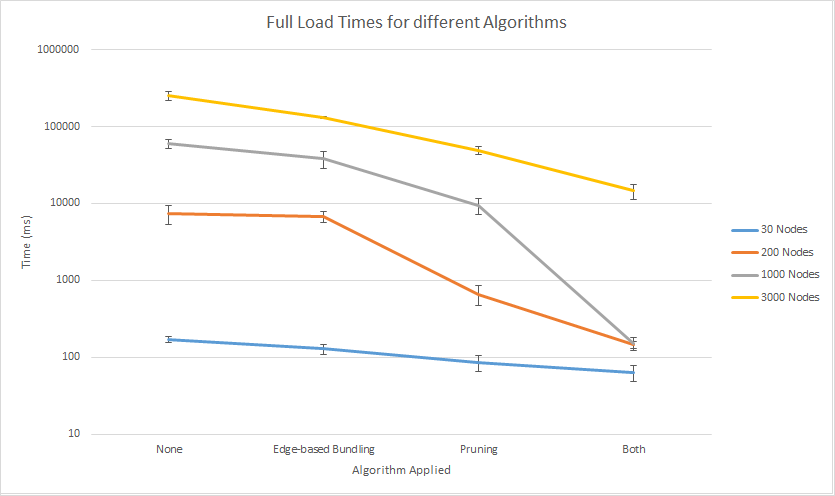
\includegraphics[width=15cm]{8/loadTimes}
    \caption{Load Times}
    \label{fig:loadTimes}
\end{figure}

Figure \ref{fig:packetSize} shows a steady decrease in packet size from no algorithm being applied, to node bundling based on number of edges, to node pruning, to applying node pruning then node bundling based on number of edges. It is again worth noting that the y-axis has a logarithmic scale.

\begin{figure}[H]
    \centering
    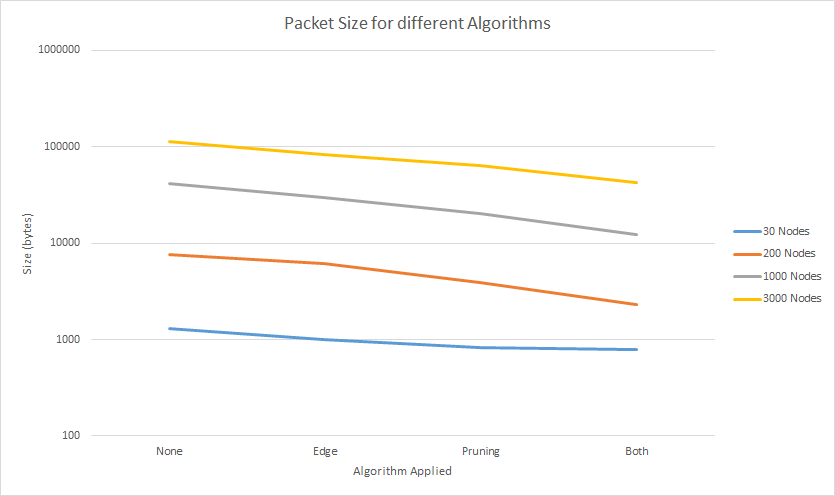
\includegraphics[width=15cm]{8/packetSize}
    \caption{Packet Size}
    \label{fig:packetSize}
\end{figure}

The above results show the benefits of applying different algorithms to reduce the amount of data that is to be visualised. This is in regards to both the amount of data that needs to be transferred, and how long it takes to load a visualisation - from a user clicking `Load' to the network rendering. 

For 30 nodes, the amount of time saved when node bundling based on edges was 41ms, and for 3000 nodes the time saved was 120759ms (just over 2 minutes). The amount of time spent processing the networks on the server in order to get the stated time savings was 0.36ms for 30 nodes and 94ms for 3000 nodes. For node pruning, the time spent pruning on the server for 30 nodes was 0.38ms and resulted in an 84.8ms speed up, and for 3000 nodes the time spent pruning on the server was 169ms and the time saved in total was 203010ms (just over 3 minutes and 20 seconds). Finally, when applying both algorithms, there was 0.42ms spent processing the information on the server for 30 nodes, with a total time saving of 107ms, and 192ms applying the algorithms on 3000 nodes, with a time saving of 237177ms (just under 4 minutes). These results clearly show the benefit of applying the bundling algorithms.

It is worth noting that, despite the fact that performance increased greatly when applying the above algorithms, this is solely due to the fact that less nodes were shown. There are attempts to reduce the amount of data lost, both in removing the programmatically decided least critical nodes to the visualisation, and showing where nodes have been bundled and how many nodes have been bundled.

The full set of results can be seen in Appendix \ref{sec:perf-eval-tab}.

\end{document}